\documentclass[oneside,a4paper,14pt]{extarticle}
\usepackage[a4paper,letterpaper,top=20mm,bottom=20mm,left=20mm,right=10mm]{geometry}
\usepackage[russian]{babel}
\usepackage{indentfirst}
\usepackage{graphicx}
\usepackage{caption}
\usepackage{titlesec}
\usepackage{minted, fancyvrb}
\usepackage{hyperref}
\usepackage{enumitem}
\usepackage{amsmath}
\usepackage{fancyhdr}
\usepackage{colortbl}
\usepackage[dvipsnames]{xcolor}
\usepackage{tikz-timing}
\usepackage{tikz}
\usetikzlibrary{karnaugh}
\usepackage{float}

% Цвета для карты Карно
\definecolor{LogisimKMapColor0}{RGB}{128,0,0}
\definecolor{LogisimKMapColor1}{RGB}{230,25,75}

% Настройка автоматических подписей к рисункам
\DeclareCaptionLabelSeparator{customdash}{~---~}
\captionsetup[figure]{name=Рисунок, labelsep=customdash, justification=centering}

% Форматирование листингов с кодом
\setminted{style = rainbow_dash, fontsize = \small} 

% Форматирование заголовков
\titleformat{\section}{\normalsize\bfseries}{\thesection}{1em}{}
\titleformat{\subsection}{\normalsize\bfseries}{\thesubsection}{1em}{}
\titleformat{\subsubsection}{\normalsize\bfseries}{\thesubsubsection}{1em}{}

% Интерлиньяж и абзац
\renewcommand\baselinestretch{1.33}
\setlength{\parindent}{1.25cm}

% Для всех списков
\setlist[enumerate]{
  left=0.5\parindent,    
  label=\arabic*.,       
  itemsep=0pt,           
  topsep=5pt,            
  partopsep=0pt,         
  parsep=0pt             
}
\setlist[itemize]{
  left=0.5\parindent,    
  itemsep=0pt,           
  topsep=5pt,            
  partopsep=0pt,
  parsep=0pt
}

% Гиперссылки
\hypersetup{
  colorlinks=true,
  linkcolor=black,
  urlcolor=blue,
  pdfborder={0 0 0},
  pdftitle={Синтез 4-разрядных счётчиков},
  pdfauthor={Черкасов А.А.},
}

\begin{document}

\newpage
\thispagestyle{empty}
\begin{center}
  МИНИСТЕРСТВО НАУКИ И ВЫСШЕГО ОБРАЗОВАНИЯ РОССИЙСКОЙ ФЕДЕРАЦИИ\\
  ФЕДЕРАЛЬНОЕ ГОСУДАРСТВЕННОЕ БЮДЖЕТНОЕ УЧРЕЖДЕНИЕ ВЫСШЕГО ОБРАЗОВАНИЯ\\
  <<ВЯТСКИЙ ГОСУДАРСТВЕННЫЙ УНИВЕРСИТЕТ>>\\
  Институт математики и информационных систем\\
  Факультет автоматики и вычислительной техники\\
  Кафедра электронных вычислительных машин
\end{center}
\vspace{10mm}

\hfill
\begin{tabular}{l}
  \footnotesize Дата сдачи на проверку:                                          \\
  \footnotesize <<\rule[-1mm]{5mm}{0.10mm}\/>>\rule[-1mm]{20mm}{0.10mm}\ 2026 г. \\
  \footnotesize Проверено:                                                       \\
  \footnotesize <<\rule[-1mm]{5mm}{0.10mm}\/>>\rule[-1mm]{20mm}{0.10mm}\ 2026 г. \\
\end{tabular}
\vfill

\begin{center}
  Отчёт по контрольной работе\\
  <<Синтез 4-разрядных счётчиков с различной организацией переноса>>\\
  по дисциплине\\
  <<Цифровая схемотехника>>\\
\end{center}
\vspace{25mm}
\noindent
\begin{tabular}{ll}
  Разработал студент гр. ИВТб-2301-05-00 & \hspace{20mm}\rule[-1mm]{30mm}{0.10mm}\,/Черкасов А.А./ \\
                                 & \hspace{27.5mm}\footnotesize(подпись)                   \\
  Преподаватель                  & \hspace{20mm}\rule[-1mm]{30mm}{0.10mm}\,/Мельцов В. Ю./  \\
                                 & \hspace{27.5mm}\footnotesize(подпись)                   \\
\end{tabular}

\noindent
\begin{tabular}{lp{58mm}r}
  Работа защищена &  & \hspace{8mm}<<\rule[-1mm]{8mm}{0.10mm}\/>>\rule[-1mm]{38mm}{0.10mm}\ 2026 г.
\end{tabular}
\vfill

\begin{center}
  Киров\\
  2026
\end{center}

\newpage\thispagestyle{plain}

\section{Цель работы}
Получить практические навыки проектирования последовательностных цифровых устройств. Выполнить теоретический логический синтез и сравнительное исследование схем 4-разрядных двоичных счётчиков трёх архитектур: асинхронного, синхронного со сквозным переносом и синхронного с параллельным переносом.

\section{Общая структура и алгоритм функционирования}
Независимо от внутренней архитектуры коммутации триггеров, внешний интерфейс (УГО) и алгоритм счёта суммирующего 4-разрядного счётчика идентичны. Устройство выполняет перебор $2^4 = 16$ состояний (от \texttt{0000} до \texttt{1111}) под воздействием тактовых импульсов $CLK$.

\begin{figure}[H]
  \centering
  \begin{tikzpicture}[thick]
    \draw (0,0) rectangle (2.5,4);
    \node at (1.25,3.5) {CT2};
    \draw (-0.5, 0.5) -- (0, 0.5); \node[right] at (0, 0.5) {$CLR$};
    \draw (-0.5, 3) -- (0, 3);
    \draw (0,2.8) -- (0.2,3) -- (0,3.2); 
    \node[right] at (0.2, 3) {$CLK$};
    \draw (2.5, 3) -- (3, 3) node[right] {$Q_0$};
    \draw (2.5, 2.25) -- (3, 2.25) node[right] {$Q_1$};
    \draw (2.5, 1.5) -- (3, 1.5) node[right] {$Q_2$};
    \draw (2.5, 0.75) -- (3, 0.75) node[right] {$Q_3$};
  \end{tikzpicture}
  \caption{Универсальное УГО 4-разрядного счётчика}
\end{figure}

\begin{center}
  Таблица 1 --- Универсальная таблица переходов счётчика \\
  \vspace{3mm}
  \resizebox{0.9\textwidth}{!}{
  \begin{tabular}{cc|cccc|cccc}
    $CLR$ & $CLK$ & $Q_3(t)$ & $Q_2(t)$ & $Q_1(t)$ & $Q_0(t)$ & $Q_3(t+1)$ & $Q_2(t+1)$ & $Q_1(t+1)$ & $Q_0(t+1)$ \\
    \hline
    0 & X & X & X & X & X & 0 & 0 & 0 & 0 \\
    \hline
    1 & $\downarrow$ & 0 & 0 & 0 & 0 & 0 & 0 & 0 & 1 \\
    1 & $\downarrow$ & 0 & 0 & 0 & 1 & 0 & 0 & 1 & 0 \\
    1 & $\downarrow$ & 0 & 0 & 1 & 0 & 0 & 0 & 1 & 1 \\
    1 & $\downarrow$ & 0 & 0 & 1 & 1 & 0 & 1 & 0 & 0 \\
    1 & $\downarrow$ & 0 & 1 & 0 & 0 & 0 & 1 & 0 & 1 \\
    1 & $\downarrow$ & 0 & 1 & 0 & 1 & 0 & 1 & 1 & 0 \\
    1 & $\downarrow$ & 0 & 1 & 1 & 0 & 0 & 1 & 1 & 1 \\
    1 & $\downarrow$ & 0 & 1 & 1 & 1 & 1 & 0 & 0 & 0 \\
    1 & $\downarrow$ & 1 & 0 & 0 & 0 & 1 & 0 & 0 & 1 \\
    1 & $\downarrow$ & 1 & 0 & 0 & 1 & 1 & 0 & 1 & 0 \\
    1 & $\downarrow$ & 1 & 0 & 1 & 0 & 1 & 0 & 1 & 1 \\
    1 & $\downarrow$ & 1 & 0 & 1 & 1 & 1 & 1 & 0 & 0 \\
    1 & $\downarrow$ & 1 & 1 & 0 & 0 & 1 & 1 & 0 & 1 \\
    1 & $\downarrow$ & 1 & 1 & 0 & 1 & 1 & 1 & 1 & 0 \\
    1 & $\downarrow$ & 1 & 1 & 1 & 0 & 1 & 1 & 1 & 1 \\
    1 & $\downarrow$ & 1 & 1 & 1 & 1 & 0 & 0 & 0 & 0 \\
  \end{tabular}
  }
\end{center}

\newpage
\section{Синтез логических уравнений счётчика}
На основании таблицы переходов составим совершенные дизъюнктивные нормальные формы (СДНФ) для функций переходов каждого разряда $Q_i(t+1)$, выбирая наборы, на которых функция принимает значение логической единицы.

\subsection{Канонические уравнения (КУ)}
\begin{align*}
  Q_0(t+1) = {} & (\overline{Q}_3\overline{Q}_2\overline{Q}_1\overline{Q}_0 \vee \overline{Q}_3\overline{Q}_2Q_1\overline{Q}_0 \vee \overline{Q}_3Q_2\overline{Q}_1\overline{Q}_0 \vee \overline{Q}_3Q_2Q_1\overline{Q}_0 \vee \\
                & Q_3\overline{Q}_2\overline{Q}_1\overline{Q}_0 \vee Q_3\overline{Q}_2Q_1\overline{Q}_0 \vee Q_3Q_2\overline{Q}_1\overline{Q}_0 \vee Q_3Q_2Q_1\overline{Q}_0) \\[2mm]
  Q_1(t+1) = {} & (\overline{Q}_3\overline{Q}_2\overline{Q}_1Q_0 \vee \overline{Q}_3\overline{Q}_2Q_1\overline{Q}_0 \vee \overline{Q}_3Q_2\overline{Q}_1Q_0 \vee \overline{Q}_3Q_2Q_1\overline{Q}_0 \vee \\
                & Q_3\overline{Q}_2\overline{Q}_1Q_0 \vee Q_3\overline{Q}_2Q_1\overline{Q}_0 \vee Q_3Q_2\overline{Q}_1Q_0 \vee Q_3Q_2Q_1\overline{Q}_0) \\[2mm]
  Q_2(t+1) = {} & (\overline{Q}_3\overline{Q}_2Q_1Q_0 \vee \overline{Q}_3Q_2\overline{Q}_1\overline{Q}_0 \vee \overline{Q}_3Q_2\overline{Q}_1Q_0 \vee \overline{Q}_3Q_2Q_1\overline{Q}_0 \vee \\
                & Q_3\overline{Q}_2Q_1Q_0 \vee Q_3Q_2\overline{Q}_1\overline{Q}_0 \vee Q_3Q_2\overline{Q}_1Q_0 \vee Q_3Q_2Q_1\overline{Q}_0) \\[2mm]
  Q_3(t+1) = {} & (\overline{Q}_3Q_2Q_1Q_0 \vee Q_3\overline{Q}_2\overline{Q}_1\overline{Q}_0 \vee Q_3\overline{Q}_2\overline{Q}_1Q_0 \vee Q_3\overline{Q}_2Q_1\overline{Q}_0 \vee \\
                & Q_3\overline{Q}_2Q_1Q_0 \vee Q_3Q_2\overline{Q}_1\overline{Q}_0 \vee Q_3Q_2\overline{Q}_1Q_0 \vee Q_3Q_2Q_1\overline{Q}_0)
\end{align*}

\subsection{Минимизация}
Проведём алгебраическую минимизацию полученных выражений. Группируя термы, приходим к минимальным выражениям, базирующимся на логической операции <<Исключающее ИЛИ>> (XOR):
\begin{align*}
  Q_0(t+1) &= \overline{Q}_0 \\
  Q_1(t+1) &= Q_1 \oplus Q_0 \\
  Q_2(t+1) &= Q_2 \oplus (Q_1 \cdot Q_0) \\
  Q_3(t+1) &= Q_3 \oplus (Q_2 \cdot Q_1 \cdot Q_0)
\end{align*}

Для реализации счётчика используются универсальные T-триггеры. Характеристическое уравнение T-триггера имеет вид $Q(t+1) = Q(t) \oplus T$. Сопоставляя его с минимизированными функциями переходов, получаем базовые логические уравнения функций возбуждения $T$-входов:
\begin{align*}
  T_0 &= 1 \\
  T_1 &= Q_0 \\
  T_2 &= Q_0 \cdot Q_1 \\
  T_3 &= Q_0 \cdot Q_1 \cdot Q_2
\end{align*}

Методы схемотехнической реализации данных уравнений (формирования переноса) определяют конечную архитектуру устройства.

\section{Архитектура 1: Асинхронный счётчик (волновой перенос)}
В асинхронном автомате тактовый сигнал подаётся исключительно на первый разряд. Переключение последующих триггеров инициируется фронтами сигналов предыдущих каскадов.

\subsection{Уравнения коммутации}
Входы $T$ всех триггеров фиксируются в логической <<1>>, переводя их в счётный режим. Перенос осуществляется через последовательное подключение тактовых входов $C_i$:
\begin{align*}
  T_0 &= 1, \quad C_0 = CLK \\
  T_1 &= 1, \quad C_1 = Q_0 \\
  T_2 &= 1, \quad C_2 = Q_1 \\
  T_3 &= 1, \quad C_3 = Q_2
\end{align*}

\subsection{Временная диаграмма}
\begin{figure}[H]
  \centering
  \resizebox{\textwidth}{!}{
  \begin{tikztimingtable}[timing/slope=0, timing/name/.style={font=\sffamily\Large}, x=2.5ex, y=3.5ex]
  $CLK$ & 18{1H 1L} \\
  $Q_0$ & 1L 17{2T} 1L \\
  $Q_1$ & 3L 8{4T} 1L \\
  $Q_2$ & 7L 4{8T} 1L \\
  $Q_3$ & 15L 16H 5L \\
  \extracode
  \begin{pgfonlayer}{background}
    \vertlines[gray, very thin]{1,3,5,7,9,11,13,15,17,19,21,23,25,27,29,31,33,35}
  \end{pgfonlayer}
  \end{tikztimingtable}
  }
  \caption{Асинхронное срабатывание каскадов (волновой перенос)}
\end{figure}

\subsection{Функциональная схема}
\begin{figure}[H]
  \centering
  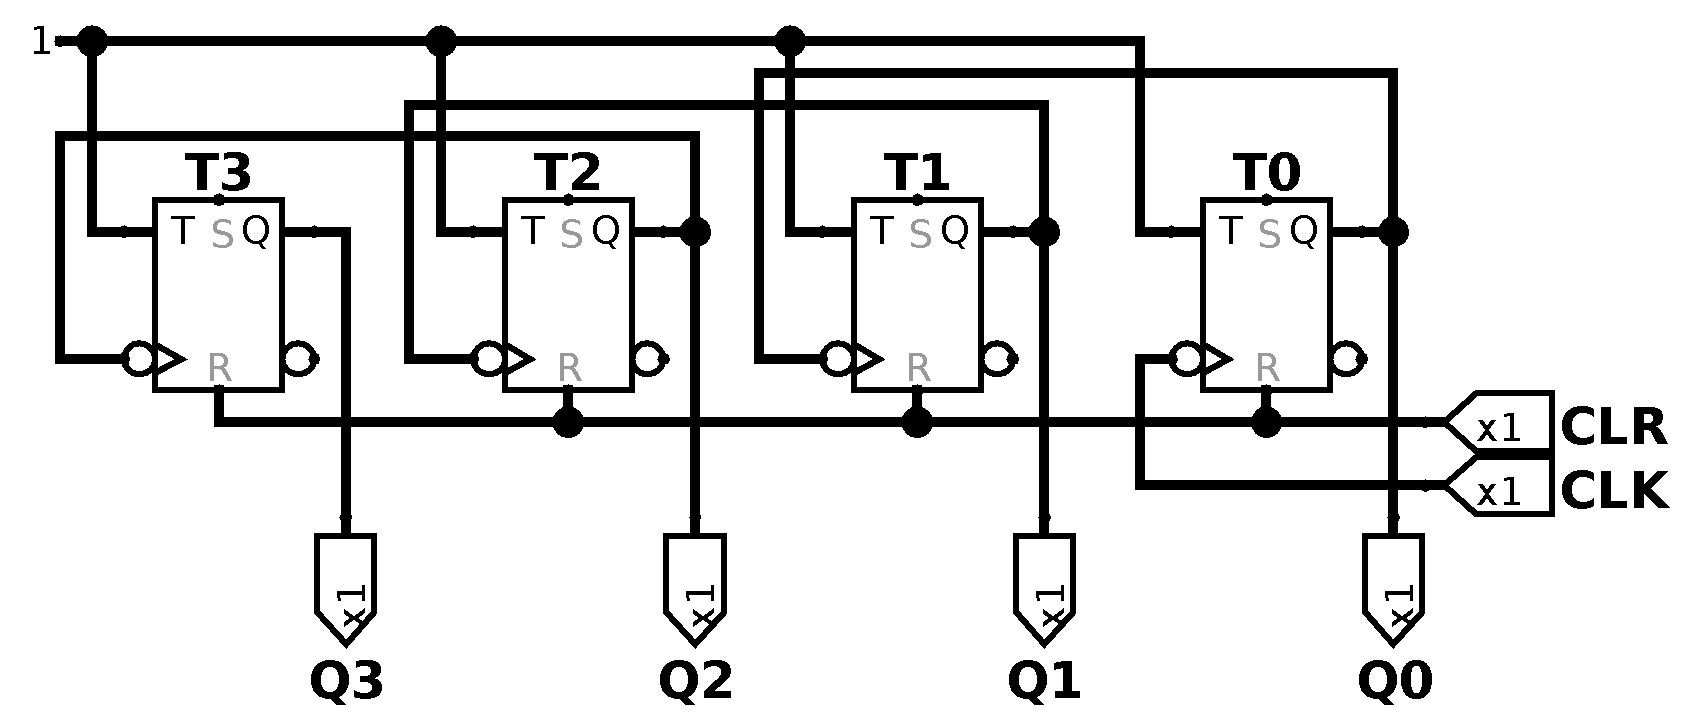
\includegraphics[width=0.95\textwidth,keepaspectratio]{pics/async.png}
  \caption{Схема электрическая функциональная асинхронного счётчика}
\end{figure}

\newpage
\section{Архитектура 2: Синхронный счётчик со сквозным переносом}
В синхронных счётчиках сигнал $CLK$ подаётся параллельно на входы $C$ всех триггеров, устраняя эффект волновой задержки переключения. Разрешение на срабатывание передаётся последовательно логическими элементами <<И>>.

\subsection{Уравнения коммутации}
Для формирования сигналов возбуждения $T_i$ вводятся промежуточные переменные сквозного переноса $P_i$. 
\begin{align*}
  C_i &= CLK \\
  P_1 &= Q_0 \quad \rightarrow \quad T_1 = P_1 \\
  P_2 &= P_1 \cdot Q_1 \quad \rightarrow \quad T_2 = P_2 \\
  P_3 &= P_2 \cdot Q_2 \quad \rightarrow \quad T_3 = P_3
\end{align*}

\subsection{Временная диаграмма}
\begin{figure}[H]
  \centering
  \resizebox{\textwidth}{!}{
  \begin{tikztimingtable}[timing/slope=0, timing/name/.style={font=\sffamily\Large}, x=2.5ex, y=3.5ex]
  $CLK$ & 18{1H 1L} \\
  $Q_0$ & 1L 17{2T} 1L \\
  $P_1$ & 1L 17{2T} 1L \\
  $Q_1$ & 3L 8{4T} 1L \\
  $P_2$ & 5L 2H 6L 2H 6L 2H 6L 2H 5L \\
  $Q_2$ & 7L 8H 8L 8H 5L \\
  $P_3$ & 13L 2H 14L 2H 5L \\
  $Q_3$ & 15L 16H 5L \\
  \extracode
  \begin{pgfonlayer}{background}
    \vertlines[gray, very thin]{1,3,5,7,9,11,13,15,17,19,21,23,25,27,29,31,33,35}
  \end{pgfonlayer}
  \end{tikztimingtable}
  }
  \caption{Формирование сквозных переносов ($P_i$) в синхронной схеме}
\end{figure}

\subsection{Функциональная схема}
\begin{figure}[H]
  \centering
  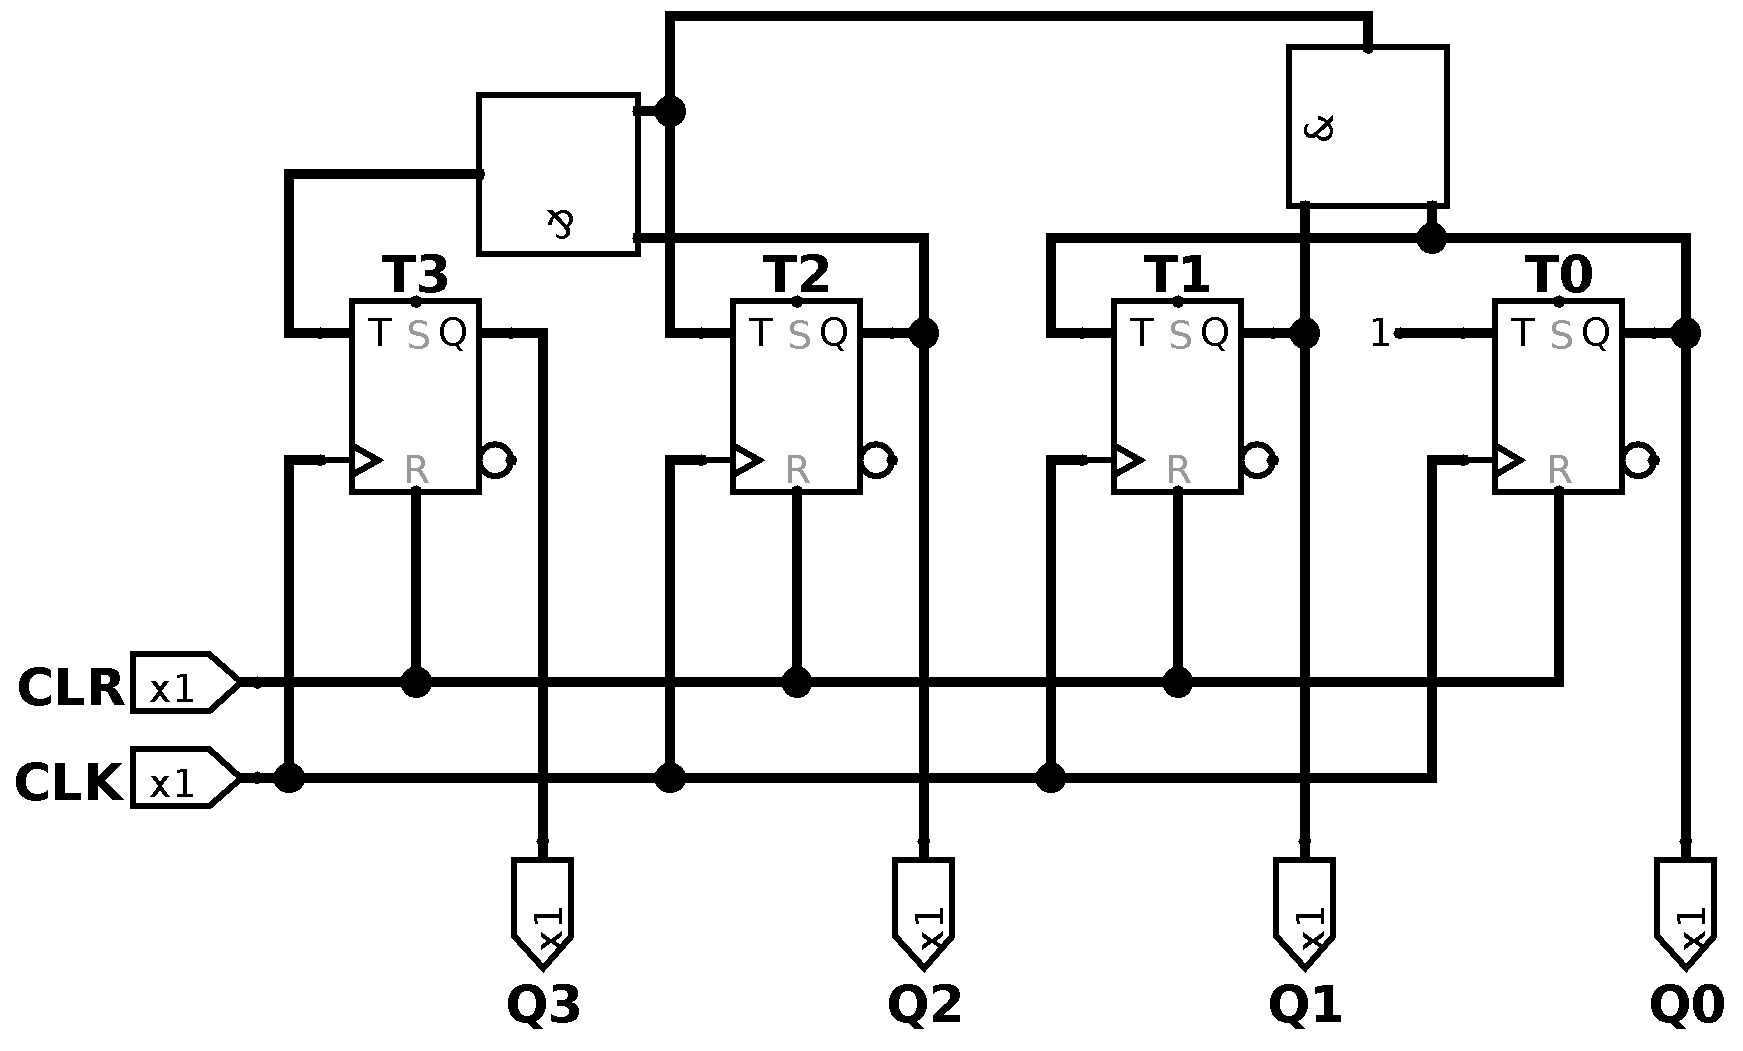
\includegraphics[width=0.95\textwidth,keepaspectratio]{pics/ripple_sync.png}
  \caption{Схема электрическая функциональная синхронного счётчика со сквозным переносом}
\end{figure}

\newpage
\section{Архитектура 3: Синхронный счётчик с параллельным переносом}
Для устранения задержек, накапливающихся при прохождении сигнала через цепочку вентилей $P_i$, применяется параллельная архитектура. Сигналы переносов формируются независимыми логическими конъюнкторами напрямую от выходов триггеров.

\subsection{Уравнения коммутации}
Система уравнений возбуждения не содержит промежуточных (каскадных) переменных:
\begin{align*}
  C_i &= CLK \\
  T_0 &= 1 \\
  T_1 &= Q_0 \\
  T_2 &= Q_0 \cdot Q_1 \\
  T_3 &= Q_0 \cdot Q_1 \cdot Q_2
\end{align*}

\subsection{Временная диаграмма}
Так как вычисления функций $T_i$ происходят параллельно, задержка формирования любого переноса $P_i$ сведена к минимуму (задержка одного вентиля <<И>>).
\begin{figure}[H]
  \centering
  \resizebox{\textwidth}{!}{
  \begin{tikztimingtable}[timing/slope=0, timing/name/.style={font=\sffamily\Large}, x=2.5ex, y=3.5ex]
  $CLK(+1)$ & 18{1H 1L} \\
  $Q_0$ & 1L 17{2T} 1L \\
  $P_1$ & 1L 17{2T} 1L \\
  $Q_1$ & 3L 8{4T} 1L \\
  $P_2$ & 5L 2H 6L 2H 6L 2H 6L 2H 5L \\
  $Q_2$ & 7L 8H 8L 8H 5L \\
  $P_3$ & 13L 2H 14L 2H 5L \\
  $Q_3$ & 15L 16H 5L \\
  \extracode
  \begin{pgfonlayer}{background}
    \vertlines[gray, very thin]{1,3,5,7,9,11,13,15,17,19,21,23,25,27,29,31,33,35}
  \end{pgfonlayer}
  \end{tikztimingtable}
  }
  \caption{Такты синхронного счётчика с параллельным переносом}
\end{figure}

\subsection{Функциональная схема}
\begin{figure}[H]
  \centering
  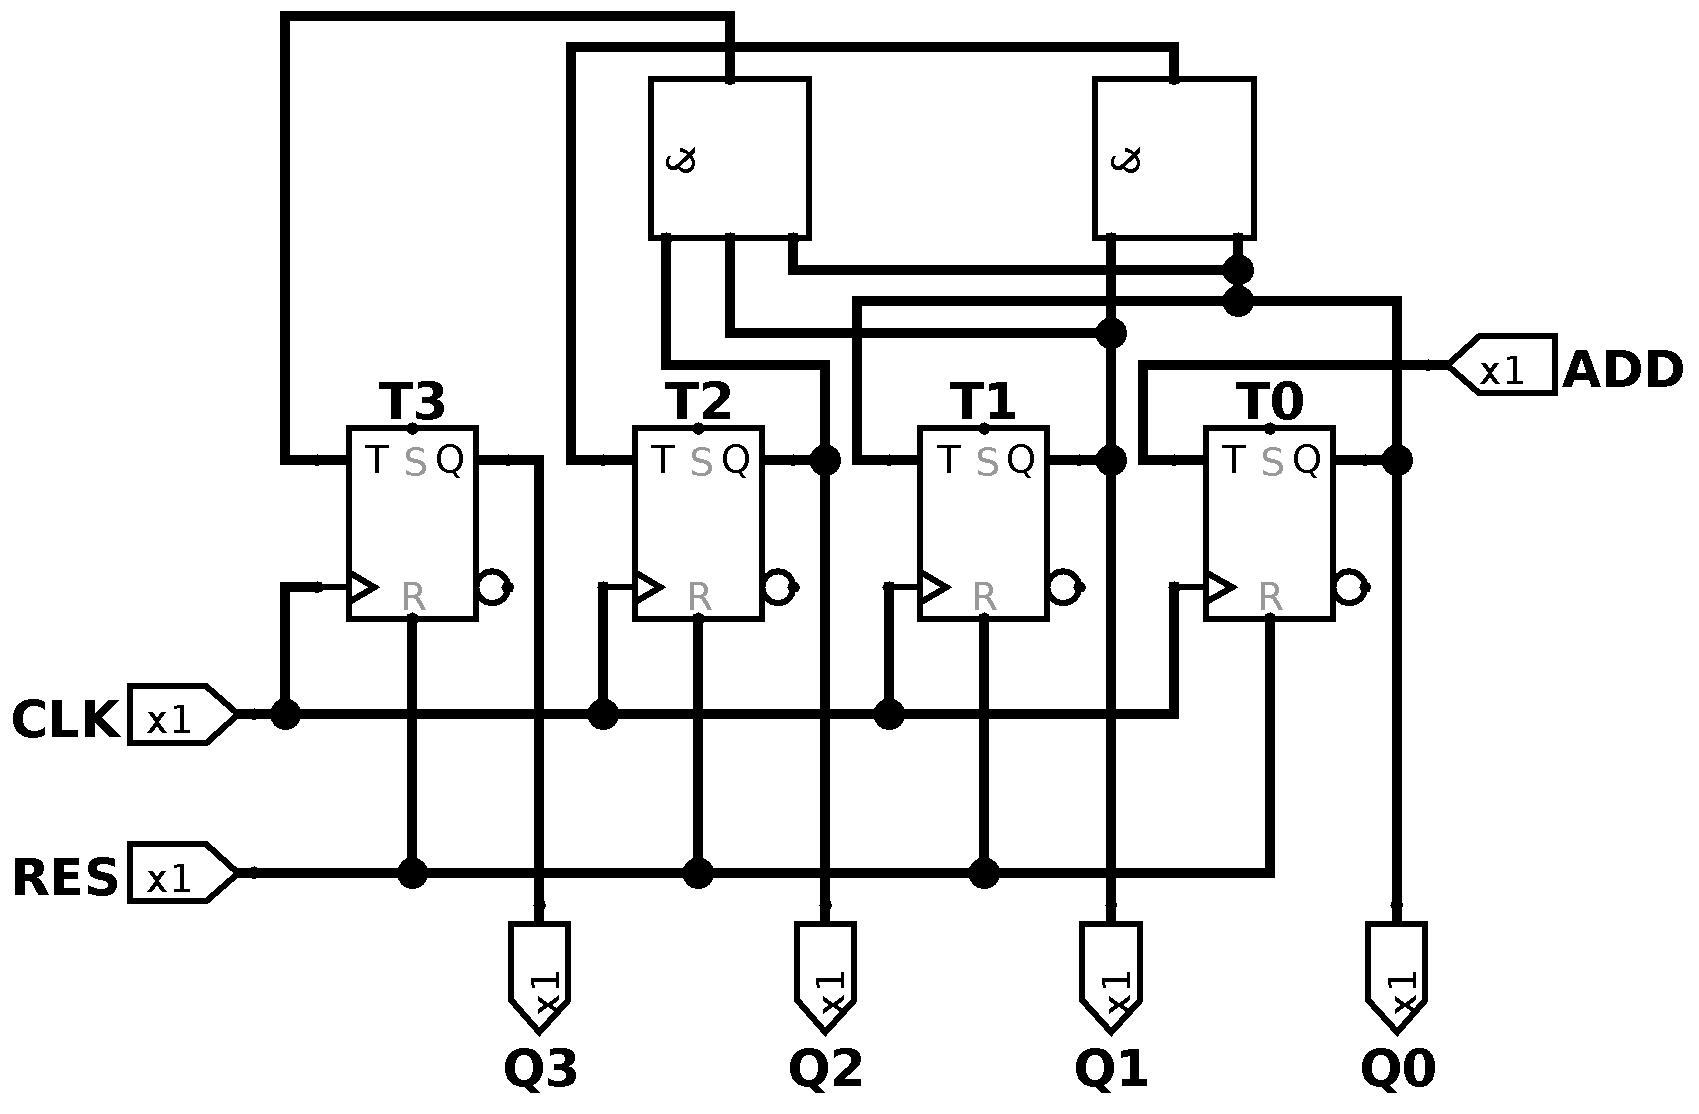
\includegraphics[width=0.95\textwidth,keepaspectratio]{pics/parallel.png}
  \caption{Схема электрическая функциональная синхронного счётчика с параллельным переносом}
\end{figure}

\section*{Вывод}
В результате выполнения контрольной работы синтезированы 4-разрядные счётчики различных архитектур. Асинхронный автомат прост в реализации, но накапливает волновые задержки. Синхронная схема со сквозным переносом решает проблему синхронизации выходов, но ограничена задержками цепочки вентилей. Оптимальным решением является счётчик с параллельным переносом, обеспечивающий независимость времени срабатывания от общей разрядности устройства.
\end{document}